\section{Lexical analyzer}
\label{Lexical analyzer}

Lexical analyzer is implemented in module \verb|lexical_analyzer.c| with the corresponding header file \verb|lexical_analyzer.h|.
The lexical analyzer decomposes source code from standard input to a sequence of tokens. A lexical analyzer has been implemented using a finite-state machine (\ref{fsm_diagram}). Individual tokens are represented by the final states.

\subsection{Implementation}
When the automaton is in the final state and is not able to process the input char, returns a token to the parser. When the automaton is not in the final state and is not able to process the input char, returns lexical error.
Each state is represented by a function. The current state is stored in global variable as pointer to the corresponding function. Next state is set in function of current state by modifying variable with pointer to current state. 
The token is represented by a structure containing information about the token type, value and flag that signs preceding eol before processed token. The value is value of a literal or the name of an identifier or flag of nilable data type and is implemented using the union data type. The token type is implemented using the enum type.

The main loop performs passage through the automaton by repeated invocation of the function referenced by the variable.
Additional global variables, that help remember information that have a lifetime longer than one state, are added in the lexical analyzer.
The communication interface with the lexical analyzer is implemented using the function \verb|get\_token()|, which has one parameter that represents a pointer to the variable to load the token into.
The Lexical analyzer has an counters (\verb|actual\_line| and \verb|actual\_column|) to tell where the error occurred.

\newpage

\subsection{Finite-state machine diagram}
\vspace*{\fill}
\begin{figure}[ht!]
\begin{center}
    \label{fsm_diagram}
    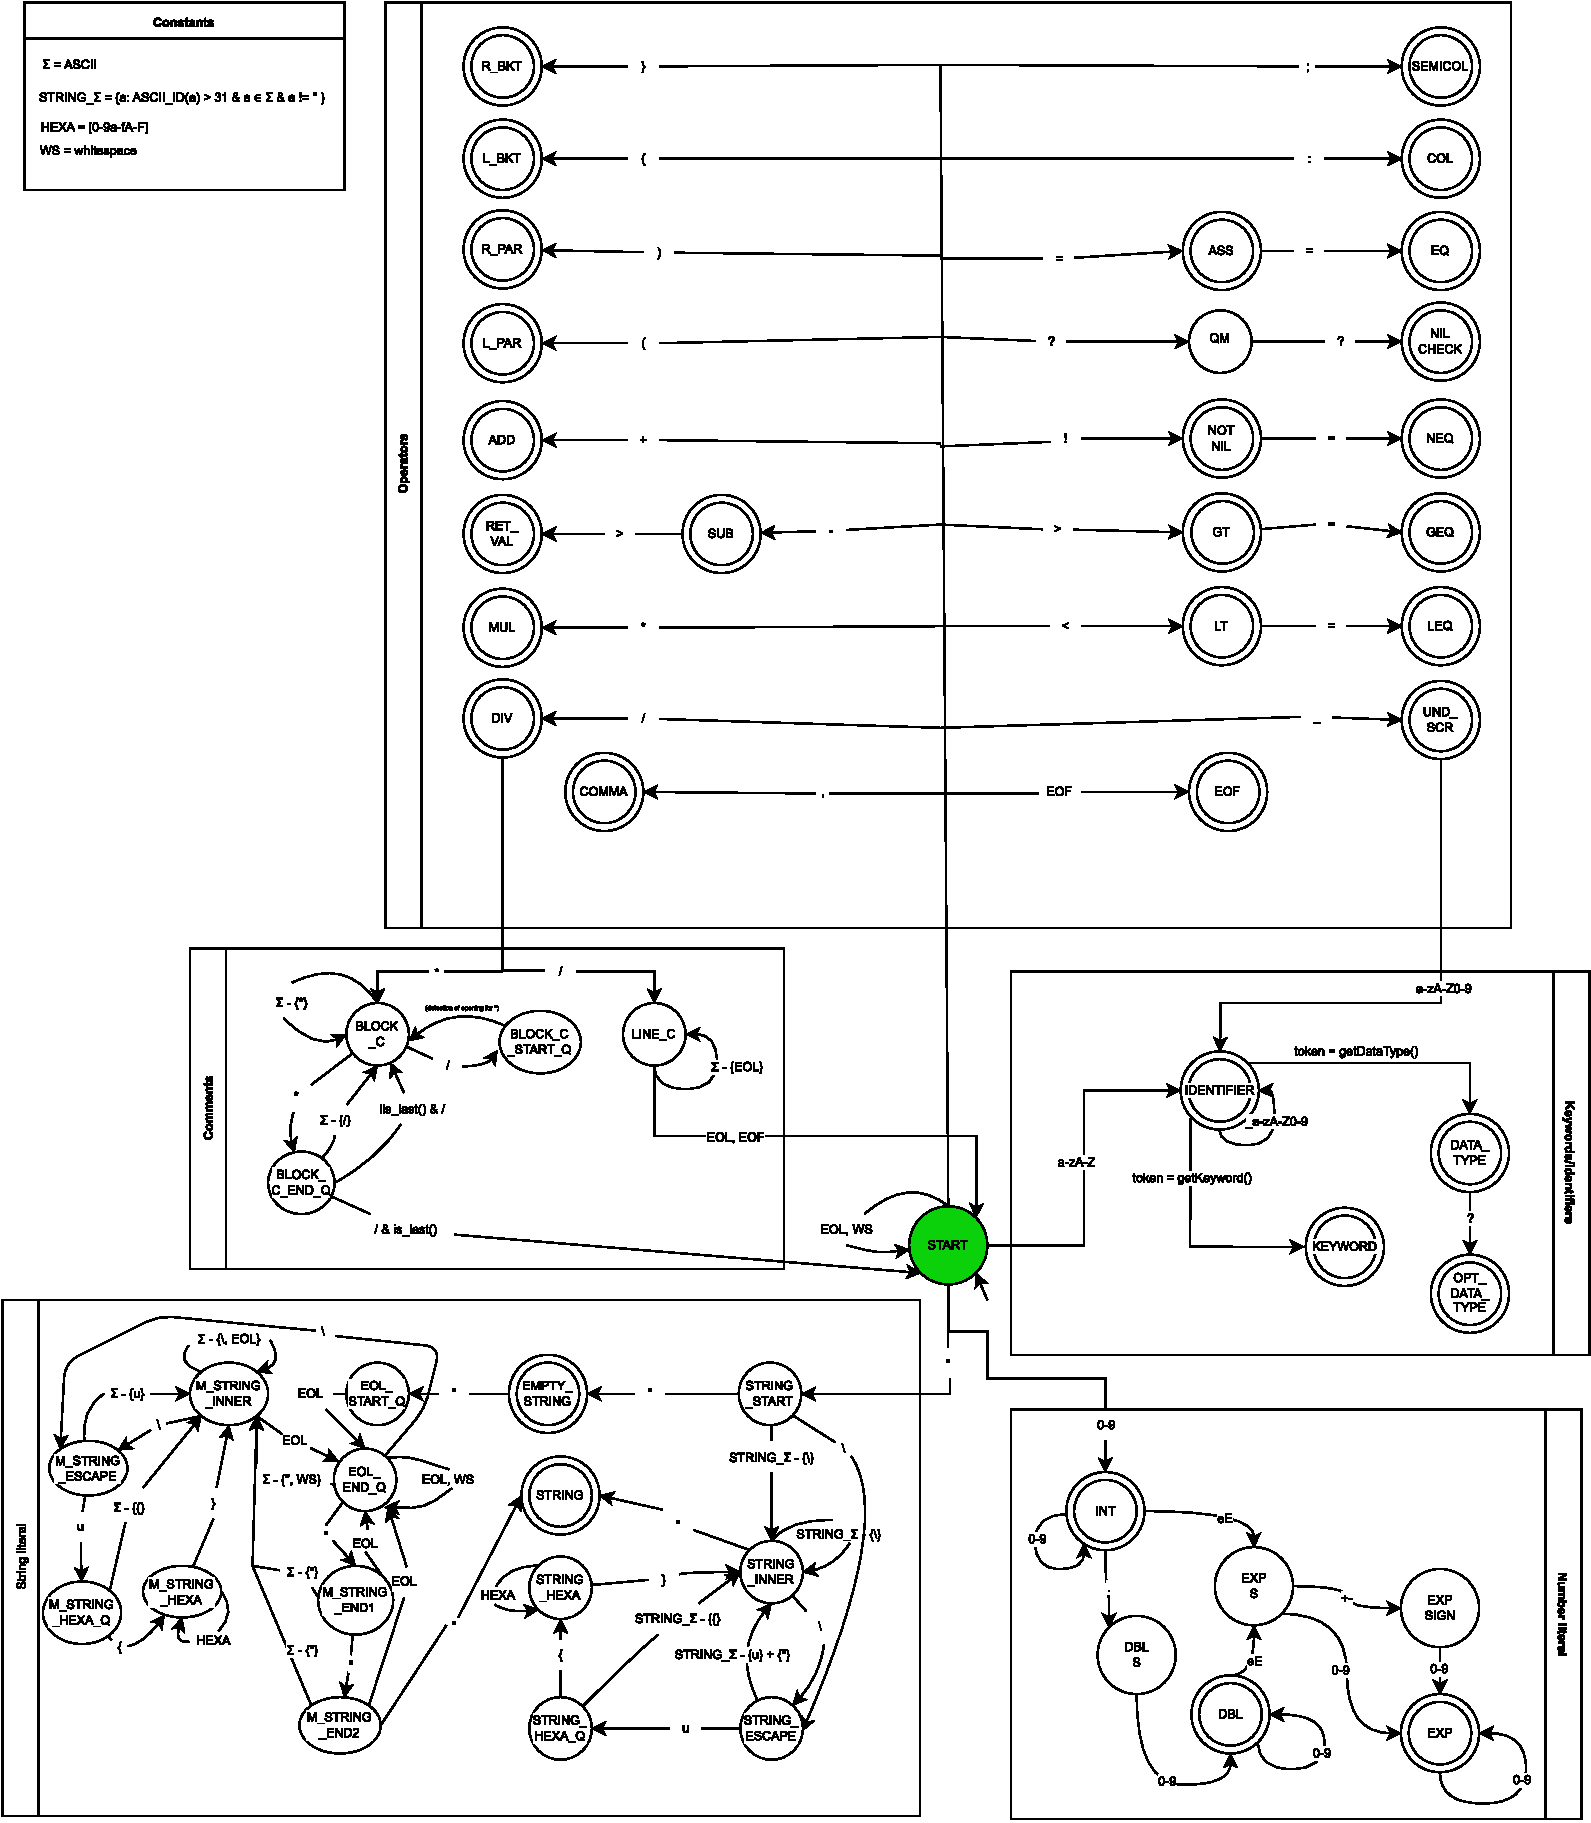
\includegraphics[width=\textwidth, keepaspectratio]{images/fsm_draft.pdf}
    \caption{Finite-state machine diagram}
\end{center}
\end{figure}
\vspace*{\fill}

\newpage